
\documentclass[twoside,twocolumn]{article}

% ------
% Fonts and typesetting settings
\usepackage[sc]{mathpazo}
\usepackage[T1]{fontenc}
\linespread{1.05} % Palatino needs more space between lines
\usepackage{microtype}
\usepackage{amsmath}
\usepackage{listings}
\usepackage{tikz}
\tikzstyle{na} = [baseline=-.5ex]
\usetikzlibrary{shapes,graphs,graphs.standard,quotes,shapes.geometric,arrows,fit,calc,positioning,automata,chains,snakes,decorations.pathreplacing}

% special tikz commands for instruction drawings
\newcommand{\tikzmark}[2]{\tikz[remember picture,baseline=(#1.base)]{\node[inner sep=2pt] (#1) {#2};}}
\tikzset{
    instrtext/.style = {font=\fontsize{25}{22.4}\selectfont},
    instrbit/.style = {font=\fontsize{20}{22.4}\selectfont}
}

%% VHDL listings
\lstdefinelanguage{VHDL}{
   morekeywords={
     library,use,all,entity,is,port,in,out,end,architecture,of,
     begin,and
   },
   morecomment=[l]--
}
\lstdefinestyle{vhdl}{
   language     = VHDL,
   basicstyle   = \ttfamily,
   keywordstyle = \color{keyword}\bfseries,
   commentstyle = \color{comment}
}
\lstset {
    basicstyle=\fontsize{7}{8}\ttfamily
}

%% caption skip
\setlength{\belowcaptionskip}{-5pt}

%% code in text
\newcommand{\code}[1]{\texttt{#1}}


% ------
% Page layout
\usepackage[hmarginratio=1:1,top=32mm,bottom=40mm,columnsep=20pt]{geometry}
\usepackage[font=it]{caption}
\usepackage{paralist}
%\usepackage{multicol}

\usepackage{graphicx}


% ------
% Lettrines
\usepackage{lettrine}

% ------
% Abstract
\usepackage{abstract}
	\renewcommand{\abstractnamefont}{\normalfont\bfseries}
	\renewcommand{\abstracttextfont}{\normalfont\small\itshape}


% ------
% Titling (section/subsection)
\usepackage{titlesec}
\renewcommand\thesection{\Roman{section}}
\titleformat{\section}[block]{\large\scshape\centering}{\thesection.}{1em}{}


% ------
% Header/footer
%\usepackage{fancyhdr}
%	\pagestyle{fancy}
%	\fancyhead{}
%	\fancyfoot{}
%	\fancyhead[C]{}
%	\fancyfoot[RO,LE]{\thepage}


\usepackage{color}

% ------
% Maketitle metadata
\title{\vspace{-7mm}%
	\fontsize{24pt}{10pt}\selectfont
	\textbf{CCOPI: Implementing a custom coprocessor interface for
    VexRiscv}
	}	
\author{%
	\large
	\textsc{Jens Nazarenus, Dominik Swierzy} \\[2mm]
	\normalsize	RheinMain University of Applied Sciences \\
    \normalsize	jens.nazarenus@hs-rm.de, dominik.swierzy@hs-rm.de
	%\vspace{-5mm}
	}
\date{\today}

\usepackage[utf8]{inputenc}

\usepackage{hyperref}


%%%%%%%%%%%%%%%%%%%%%%%%
\begin{document}

\maketitle
%\thispagestyle{fancy}

\begin{abstract}
\noindent In this paper we introduce CCOPI, a custom coprocessor interface for the
RISC-V implementation VexRiscv. CCOPI as well as VexRiscv is written in
the hardware description language SpinalHDL. The interface is responsible 
for the communication between the coprocessor and the core CPU pipeline of 
VexRiscv and thus helps hardware developers in the designing process of 
a coprocessor with a custom instruction-set extension.

CCOPI uses the flexibility of the RISC-V implementation VexRiscv to create 
the interface. This paper also shows how VexRiscv is designed particularly with 
regard to modifications and custom extensions. 
\end{abstract}

\section{Introduction}
Coprocessors in general are used to support the core CPU(s) with the
calculation of specific mathematical operations. A coprocessor aims to
accelerate this specific task over a software implementation of the same
task.

Former coprocessors like the Intel 80387 or Motorolas 68881 were used to
execute IEEE 754 compliant floating point operations and could be
bought as independent components. To use the coprocessors new
instructions were included in the instruction stream of the core CPU.

Today the logic of coprocessors are often included inside the CPU
itself as an instruction-set extension. Well-known examples are the
Intel\textregistered{} x87 
floating point unit (FPU) or the Intel\textregistered{} Advanced Encryption Standard New 
Instructions (AES-NI). Both modules introduce new instructions which can
be used by developers.
CCOPI is designed to produce coprocessors which resides inside the core
RISC-V CPU named VexRiscv similar to x87 or AES-NI discussed above.

Before approaching the main topic CCOPI and its implementation, this paper
gives an introductional overview of the topics RISC-V and the used
hardware description language SpinalHDL.
\section{RISC-V}
RISC-V is the name of an open source instruction-set architecture (ISA)
which has been developed at the University of California, Berkeley.
The ISA describes the instructions any RISC-V implementation must
implement, plus optional extensions. The required minimum is specified in
the ``Base Integer Instruction Set'' of the User Level ISA.

A RISC-V instruction $instr$ is always decoded in 32 bits.

       \begin{figure}[h]
        \centering
        \resizebox{7.25cm}{!}{
            \begin{tikzpicture}[]
                %% R-type
                \draw[] (0,6) -- (31,6);
                \draw[] (0,7) -- (31, 7);
                \draw[] (0,6) -- (0,7);
                \draw[] (31,6) -- (31,7);

                \draw[] (31-7,6) --(31-7,7);
                \draw[] (31-12,6) --(31-12,7);
                \draw[] (31-15,6) --(31-15,7);
                \draw[] (31-20,6) --(31-20,7);
                \draw[] (31-25,6) --(31-25,7);

                \node[instrtext] at (31-25-3,6.5) {funct7};
                \node[instrtext] at (31-19-3.5,6.5) {rs2};
                \node[instrtext] at (31-15-2.5,6.5) {rs1};
                \node[instrtext] at (31-12-1.5,6.5) {funct3};
                \node[instrtext] at (31-7-2.5,6.5) {rd};
                \node[instrtext] at (31-0-3.5,6.5) {opcode};

                %% bit header
                \node[instrbit] at (0+0.3,7+0.5) {31};
                \node[instrbit] at (31-7-0.3, 7+0.5) {7};
                \node[instrbit] at (31-12-0.5, 7+0.5) {12};
                \node[instrbit] at (31-12+0.5, 7+0.5) {11};
                \node[instrbit] at (31-15-0.5, 7+0.5) {15};
                \node[instrbit] at (31-15+0.5, 7+0.5) {14};
                \node[instrbit] at (31-20+0.5, 7+0.5) {20};
                \node[instrbit] at (31-20-0.5, 7+0.5) {19};
                \node[instrbit] at (31-25+0.5, 7+0.5) {24};
                \node[instrbit] at (31-25-0.5, 7+0.5) {25};
                \node[instrbit] at (31-7+0.3, 7+0.5) {6};
                \node[instrbit] at (31-0.3, 7+0.5) {0};

                %%\node[instrtext] at (33, 6.4) {R-Type};

            \end{tikzpicture}
        }

        \caption[Instruktionstypen]{R-Type instruction format}      
        \label{fig:riscv_r_type}
    \end{figure}

\noindent The notation $instr[fromBit:toBit]$ is used to extract information from
the instruction. In Figure \ref*{fig:riscv_r_type} $instr[6:0]$
represents the opcode, which is the identification code for a machine
instruction. Depending on the opcode $instr[31:7]$ is decoded in
different ways. In Figure \ref*{fig:riscv_r_type} the ``R-Type''
instruction format is shown, which is responsible for Integer-Register-Register
operations, where the operands are located in the registers specified by
$rs1$ and $rs2$. With $instr[11:7]$ the destination register $rd$ is
specified. $funct7$ and $funct3$ defines the exact sub operation of the
instruction.

       \begin{figure}[h]
        \centering
        \resizebox{7.25cm}{!}{
            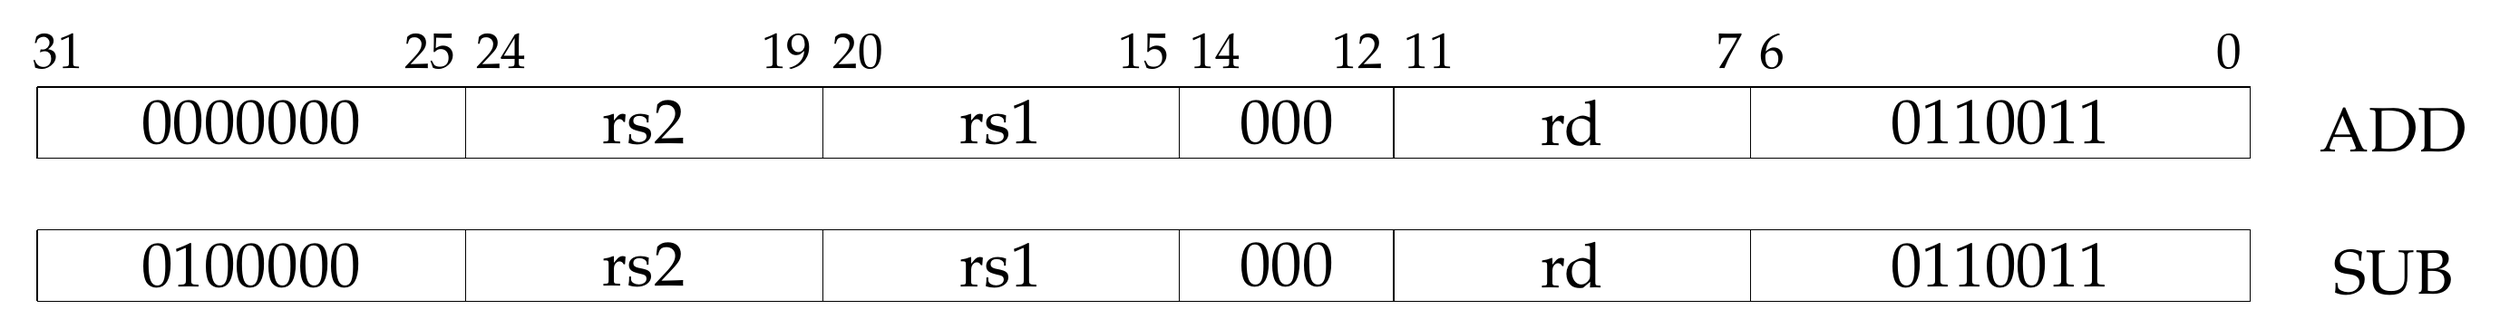
\begin{tikzpicture}[]
                % ADD
                \draw[] (0,6) -- (31,6);
                \draw[] (0,7) -- (31, 7);
                \draw[] (0,6) -- (0,7);
                \draw[] (31,6) -- (31,7);

                \draw[] (31-7,6) --(31-7,7);
                \draw[] (31-12,6) --(31-12,7);
                \draw[] (31-15,6) --(31-15,7);
                \draw[] (31-20,6) --(31-20,7);
                \draw[] (31-25,6) --(31-25,7);

                \node[instrtext] at (31-25-3,6.5) {0000000};
                \node[instrtext] at (31-19-3.5,6.5) {rs2};
                \node[instrtext] at (31-15-2.5,6.5) {rs1};
                \node[instrtext] at (31-12-1.5,6.5) {000};
                \node[instrtext] at (31-7-2.5,6.5) {rd};
                \node[instrtext] at (31-0-3.5,6.5) {0110011};

                % SUB
                \draw[] (0,4) -- (31,4);
                \draw[] (0,5) -- (31, 5);
                \draw[] (0,4) -- (0,5);
                \draw[] (31,4) -- (31,5);

                \draw[] (31-7,4) --(31-7,5);
                \draw[] (31-12,4) --(31-12,5);
                \draw[] (31-15,4) --(31-15,5);
                \draw[] (31-20,4) --(31-20,5);
                \draw[] (31-25,4) --(31-25,5);

                \node[instrtext] at (31-25-3,4.5) {0100000};
                \node[instrtext] at (31-19-3.5,4.5) {rs2};
                \node[instrtext] at (31-15-2.5,4.5) {rs1};
                \node[instrtext] at (31-12-1.5,4.5) {000};
                \node[instrtext] at (31-7-2.5,4.5) {rd};
                \node[instrtext] at (31-0-3.5,4.5) {0110011};


                %% bit header
                \node[instrbit] at (0+0.3,7+0.5) {31};
                \node[instrbit] at (31-7-0.3, 7+0.5) {7};
                \node[instrbit] at (31-12-0.5, 7+0.5) {12};
                \node[instrbit] at (31-12+0.5, 7+0.5) {11};
                \node[instrbit] at (31-15-0.5, 7+0.5) {15};
                \node[instrbit] at (31-15+0.5, 7+0.5) {14};
                \node[instrbit] at (31-20+0.5, 7+0.5) {20};
                \node[instrbit] at (31-20-0.5, 7+0.5) {19};
                \node[instrbit] at (31-25+0.5, 7+0.5) {24};
                \node[instrbit] at (31-25-0.5, 7+0.5) {25};
                \node[instrbit] at (31-7+0.3, 7+0.5) {6};
                \node[instrbit] at (31-0.3, 7+0.5) {0};




                \node[instrtext] at (33, 6.4) {ADD};
                \node[instrtext] at (33, 4.4) {SUB};

            \end{tikzpicture}
        }

        \caption[Instruktionstypen]{ADD, SUB operation}      
        \label{fig:add_sub}
    \end{figure}

\noindent Figure \ref*{fig:add_sub} shows that both the ADD and the SUB
operation share the opcode $0110011$. The field $funct7$, which is
decoded in $instr[31:25]$, exposes the exact type of operation:
\begin{itemize}
    \item 0000000 : ADD operation
    \item 0100000 : SUB operation
\end{itemize}
$rs1$, $rs2$ and $rd$ are always encoded at the same positions
in $instr$ to simplify the decoding process in an implementation of
RISC-V.

The ISA also defines opcodes which will not be used by future extensions
and can be used for custom instruction-set extensions:
    \begin{itemize}
        \item $0001011$ : custom-0
        \item $0101011$ : custom-1
        \item $1011011$ : custom-2
        \item $1111011$ : custom-3
    \end{itemize}
The opcodes of custom-2/3 may not be used in RISC-V implementations where the
integer registers are extended to 128 bits (RV128I). With CCOPI it is
possible to create instruction-set extensions with one or more of the described 
custom opcodes.
\section{SpinalHDL}
The CPU implementation VexRiscv and CCOPI are implemented in the
language ``SpinalHDL'', which is a ``high level hardware description
language'' to describe digital hardware as part of register-transfer
level design. The output of a compilation process is VHDL or
Verilog code. For this reason SpinalHDL is a transcompiler which takes
Scala code and transforms it into Verilog or VHDL.  

In the following example a Component named ``Comp'' is created. The
design adds the two input signals ``a'' and ``b'' with an additional
``x'' which is specified as a Scala class constructor parameter: 
\begin{lstlisting}[language=scala]
class Comp(x: Int) extends Component {
    val io = new Bundle {
        val a, b = in UInt(8 bits)
        val result = out UInt(8 bits)
    }
    io.result := io.a + io.b + x
}
\end{lstlisting}
To generate the module, the compiler of SpinalHDL gets called with one of
the functions \code{SpinalVerilog(component)} or
\code{SpinalVhdl(component)}. The variable ``x'' is set to $15$:
\begin{lstlisting}[language=scala]
object MyComponentGen {
  def main(a: Array[String]): Unit = {
    SpinalVerilog(new Comp(15))
  }
}
\end{lstlisting}
Afterwards the following Verilog code gets emitted in the file
``Comp.v'', where $15$ is resolved to \code{8’b00001111} by the
SpinalHDL compiler.
\begin{lstlisting}[language=verilog]
module Comp (
      input  [7:0] io_a,
      input  [7:0] io_b,
      output [7:0] io_result);
  wire [7:0] zz_1;
  assign zz_1 = (io_a + io_b);
  assign io_result = (zz_1 + 
                     (8'b00001111));
endmodule
\end{lstlisting}
With the combination of Scala and SpinalHDL it is possible to create
more abstract hardware designs. It is also possible to use object
oriented software patterns like inheritance, polymorphism or type
parametrization. Even higher-order functions like Scalas ``map''
function will get evaluated during the compilation.

The following SpinalHDL code initializes a ROM with predefined values in
a Scala list:
\begin{lstlisting}[language=scala]
def sbox = List(0x63, 0x7C, ...)
val romsbox = Mem(Bits(8 bits), 
                  sbox.map(B(_, 8 bits)))
\end{lstlisting}

\noindent The generated code looks like this:
\begin{lstlisting}[language=verilog]
module Comp ();
  reg [7:0] romsbox [0:1];
  initial begin
    romsbox[0] = 'b01100011;
    romsbox[1] = 'b01111100;
    ...
  end
endmodule
\end{lstlisting}
SpinalHDL also introduces data types which are divided in Composite
types and Base types. The available Base types are:
\begin{itemize}
    \item Bool (True, False)
    \item Bits (A vector of Bits, like \code{B"0011"})
    \item UInt/SInt (Unsigned/Signed Integer, used for integer
        arithmetic)
\end{itemize}
Composite types are supposed to group Base types. A \code{Bundle} for
example may be used to group the available input/output signals of a
component under a single name:
\begin{lstlisting}[language=scala]
val io = new Bundle {
    val a, b = in UInt(8 bits)
    val result = out UInt(8 bits)
}
\end{lstlisting}
Since SpinalHDL is based on Scala, build tools like SBT can be used to
manage dependencies and compile a SpinalHDL based hardware project. The
dependencies \code{spinalhdl-core} and \code{spinalhdl-lib} are required
to use language features discussed above.
\begin{lstlisting}[language=scala]
libraryDependencies ++= Seq(
  "com.github.spinalhdl" % "spinalhdl-core_2.11" 
    % "0.10.15",
  "com.github.spinalhdl" % "spinalhdl-lib_2.11" 
    % "0.10.15",
)
\end{lstlisting}

Both VexRiscv and CCOPI use the object oriented design pattern paired
with functional programming elements to describe the hardware in an
abstract way. The next chapter gives a more detailed overview of the
RISC-V implementation named VexRiscv.

\section{VexRiscv}
CCOPI uses VexRiscv as its underlying RISC-V implementation. VexRiscv 
implements the ``RV32IM'' instruction set, which means:
\begin{itemize}
    \item 32 Bit registers
    \item Base Integer instruction set
    \item Standard Extension for Integer
Multiplication and Division
\end{itemize}
The CPU is pipelined on a five-stage RISC pipeline like the MIPS
architecture. The \textbf{Instruction Fetch} stage is responsible of
writing the next 32-bit instruction in the register ``pc''. Afterwards
the \textbf{Decode} stage analyzes the instruction. Based on the opcode
the decode stage knows to interpret $instr[31:7]$ of the instruction
which is stored in ``pc''. The \textbf{Execute} stage computes a result
based on the operands which were determined in the Decode stage. The
Execute stage consists of multiple Arithmetic Logical Units (ALU) to
perform arithmetic or logical operations. The \textbf{Memory} stage
handles the Load/Store operations of RISC-V. The last pipeline stage,
the \textbf{Write Back} stage, copies the result of the Execute stage in
the destination register ``rd'', which is specified in $instr[11:7]$ of
the instruction.
\subsection{Plugin mechanism}
\section{CCOPI}
\section{Acceleration Evaluation}

\bibliographystyle{unsrt}
\bibliography{literature}

\end{document}
